\documentclass{article}
\usepackage[utf8]{inputenc}
\usepackage[margin=1.25in]{geometry}
\usepackage{amsmath}
\usepackage{ amssymb }
\usepackage{ dsfont }
\usepackage{setspace}
\usepackage{graphicx}
\usepackage{physics}
\usepackage{subcaption}
\graphicspath{ {pix/} }

\title{Computational Physics 3}
\author{Jack Donahue}
\begin{document}


\maketitle
\doublespacing

\begin{abstract}
In this report we write our first hydrodynamics code and put it through some initial test. The methods used are first and higher order HLL approximate Riemann solver. These methods are applied to the test problems of the sod shock tube and an isentropic wave. Convergence rates are the calculated and compared to theorertical predictions.
\end{abstract}
\section*{Introduction}

When writing hydrodynamics code, it is desirable to focus on conserved quantities in the problem. Without such an approach, code can run into problems of run away energy and density to name a few. With such a focus, we only need to find the flux between cells to calculate how much the conserved quantities change in each cell. This is a consequence of the fact that we're dealing with conserved quantities without source terms, so 
\begin{equation}
    \frac{df}{dt}= - \int_{S} f \cdot dS.
\end{equation}
The problem of calculating fluxes between two regions of different state variables is generally described by the Riemann problem. Remarkably, this problem has been solved analytically and so our approach is made tractable. The exact solution is iterative, however, so can be expensive computationally. Researchers in computational fluid dynamics have been finding more efficient approximate methods for decades. We will use one called HLL (Harten-Lax-van Leer) solver given by 
\begin{equation}
    F^{HLL} = \frac{\alpha^+ F^{L}+\alpha^- F^{R} - \alpha^+ \alpha^- (U^{L} - U^{L})}{\alpha^+ + \alpha^-},
\end{equation}
where R and L denote the states to the left and to the right of the boundary. Here, $\alpha^+$ and $\alpha^-$ are given by the eigenvalues of the Jacobians of the left and right states as
\begin{equation}
    \alpha^{\pm} = \mbox{MAX}(0,\pm \lambda^\pm(U^{L}),\pm \lambda^\pm(U^{R}) ).
\end{equation}
This for calculating fluxes gives both accurate and quick results by reducing the problem to the important initial shock and rarefaction. More complex approximate methods take into account the contact discontinuity and further features, but those will not be considered here for this simple application. 

\section*{Method}

\subsection*{First Order}

In the first order approximation, we will simply discretize our space into $N$ pieces and set out time step by the Courant condition $\Delta t < \Delta x/\mbox{MAX}(\alpha^\pm)$. Fluxes at the boundaries will be given by the HLL solver above, and so the time change for a cell $i$ at time step $n$ will be 
\begin{equation}
    \frac{dU^n_i}{dt} = L(U^n_i) = -\frac{F^n_{i+1/2} - F^n_{i-1/2}}{\Delta x}, 
\end{equation}
where $i\pm1/2$ denote the boundaries of the cell. The future time step of the cell will then be given by $U^{n+1}= U^n + \Delta t \cdot L(U^n) $. 

This first order method will be tested against the sodshock problem. The set up is a one dimensional line of gas with constant left and right states of some boundary in the middle. This is identical to the basic Riemann solver so can be compared directly to the results obtained from the analytic solution and the convergence rate found. 

\subsection*{Higher Order}

We will then move to compute higher order in space and time. The time evolution will be updated with a third-order Runge-Kutta method. This method is given by

\begin{equation}
    U^{(1)}= U^n + \Delta t \cdot L(U^n),
\end{equation}
\begin{equation}
    U^{(2)}= \frac{3}{4}U^n + \frac{1}{4}U^{(1)}+ \frac{1}{4}\Delta t \cdot L(U^{(1)}),
\end{equation}
\begin{equation}
    U^{n+1}= \frac{1}{3} U^n + \frac{2}{3}U^{(2)} + \frac{2}{3} \Delta t \cdot L(U^{(2)}).
\end{equation}

We will also increase our resolution in space by interpolating between the values of $U^n_i$. This interpolation is given by a piecewise linear method with a generalized minmod slope limiter. The state vector $U^n$ is given at the middle of each cell $i$, so this method will give us approximations to the solutions closer to either side of the boundary. With a boundary (plus one) for every cell, this doubles the number of states we have to calculate the flux from. This interpolation is repeated every time step and are only used to better approximate fluxes. 

The discontinuities of the sodshock will hide the improvements of the higher order hydrodynamics code. Instead, we will test it on a smooth isentropic wave. These waves will steepen and form a shock at late times, so we will restrict to earlier times. Error in our method will calculated from the change in specific entropy, 
\begin{equation}
    s(x,t) - s_0 = \frac{1}{\gamma -1} \log\bigg[\frac{P(x,t)}{P_0}\bigg(\frac{\rho(x,t)}{\rho_0}\bigg)^{-\gamma} \bigg].
\end{equation}
In the analytic solution to the isentropic wave, this value is zero for all time and space. 

\section*{Results}

Convergence plots of the first order method on the sodshock problem are presented in Figure \ref{fig:onedimconv} and a sample waveform with N=1000 in Figure \ref{fig:onedimex}. Convergence rates for different values of the state vector were different, but were in the range of .6 to .8. 

The convergence plots for the higher order method to the problem of the isentropic wave are presented in Figure \ref{fig:highorconv}. Convergence rates for the higher dimensional code were found to be 2.4. Example wave forms for this higher order method are found in Figure \ref{fig:highordex} for N=1000 cells. 
  
\section*{Discussion}

The first order method does surprisingly well in capturing the main features of the sodshock. As we can see in Figure \ref{fig:onedimex}, The initial shock and rarefaction fan are very well represented. The contact discontinuity is smeared out, a characteristic of the HLL script which averages over density discontinuities between cells. 

The convergence rates vary because the HLL is good at capturing some things more than others. We noted in lecture that one would have to use HLLC to more accurately capture the features of the contact discontinuity, a change in the density. We see in Figure \ref{fig:onedimconv} that in fact the density converges the slowest, in line with the conclusion that standard HLL is not as good at capturing abrupt density changes. We expected theoretically that the convergence should be of order 1, but we observe rates less than 1 for all state variables. This could be partly due to the approximate HLL solver, but also to the sharp discontinuities in the initial problem. 

As expected, the high order method fits the smooth isentropic wave extremely well. As we can see in Figure \ref{fig:highordex}, the two are indistinguishable by eye from each other. More interesting are the convergence rates. We find, using specific entropy measure described in Methods, that the higher order method converges at a rate of 2.4. This is a bit better than the second order that we expected. Although we could speculate to the origin of this, sometimes it's better to just accept better than expected results than to interrogate them too viciously. 


\section*{Conclusion}

The first-order method did quite well on the sodshock problem when compared visually. The convergence rate, however, left something to be desired. It would be interesting to implement a HLLC to directly see the improvement in resolving the contact discontinuity. 

The high-order is much better and converges much more quickly than the first order, as expected. It would be instructive to run this code out until a shock forms to test the limits of the code. We also hope to study higher order methods in space and time in the future. 


\begin{figure}[h]
    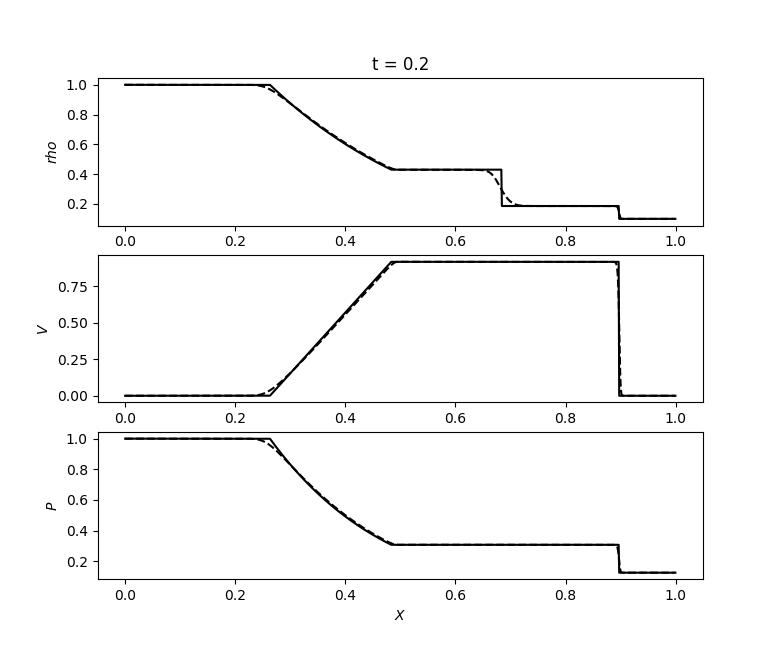
\includegraphics[width=\textwidth]{onedimex1000.png}
    \caption{Example plot waveforms for the sodshock problem with a first-order HLL method, N=1000. The solid line is the analytic solution and the dashed the first order method approximation. }
    \label{fig:onedimex}
\end{figure}

\begin{figure}[h]
    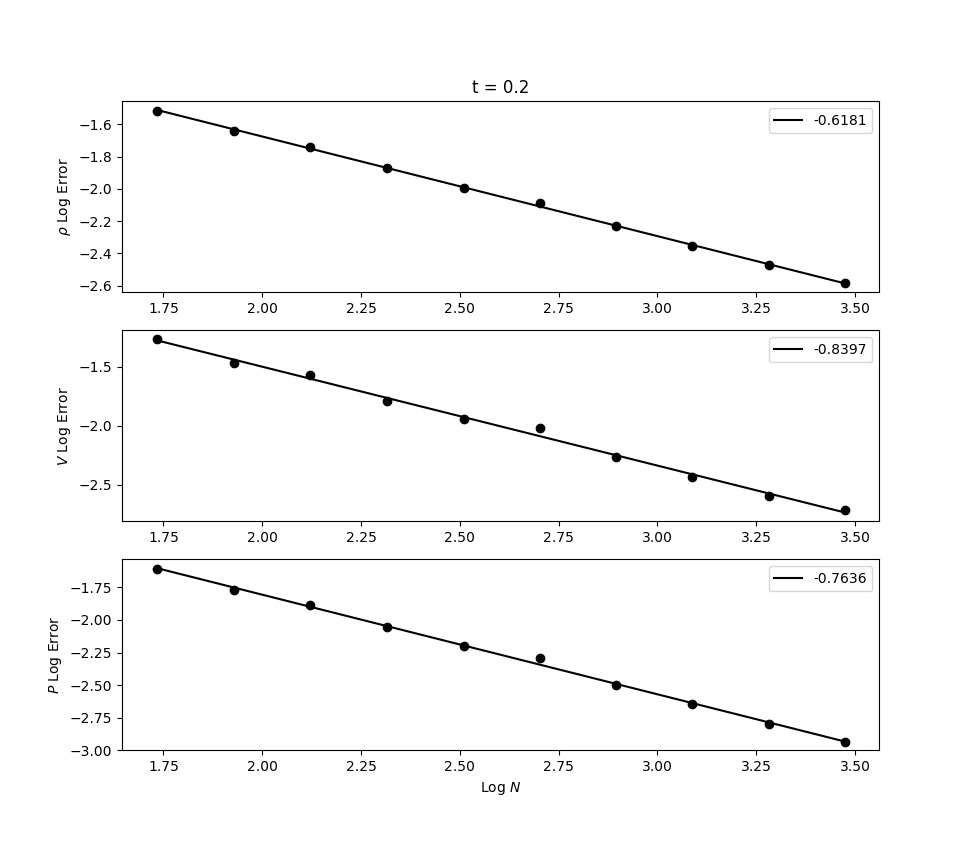
\includegraphics[width=\textwidth]{onedimerror.png}
    \caption{Convergence rate graphs for the first order method with HLL on the problem of the sodshock. Given in the upper right of each graph is best fit slope.}
    \label{fig:onedimconv}
\end{figure}

\begin{figure}[h]
    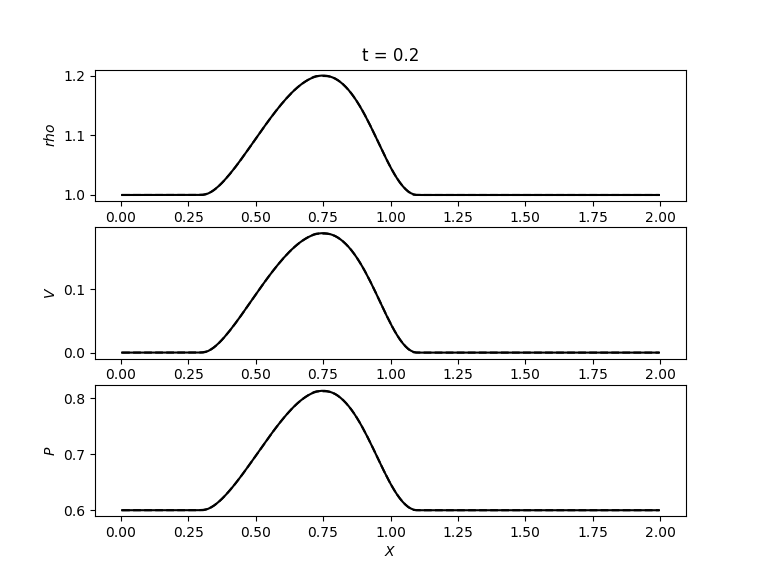
\includegraphics[width=\textwidth]{highorderex.png}
    \caption{Example state for the higher order method, with N=1000 test points. The analytic solution and the approximate are laying on top of each other, with the difference being slightly visible at the peak of the wave.}
    \label{fig:highordex}
\end{figure}

\begin{figure}[h]
    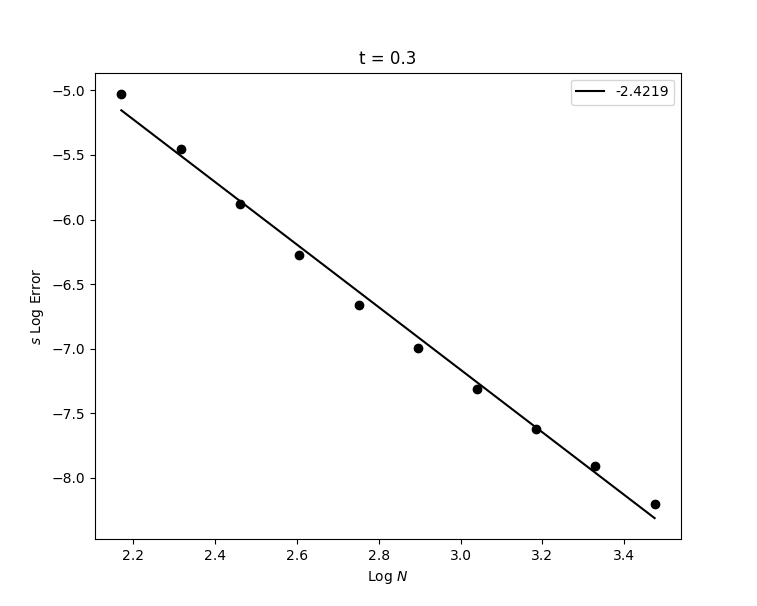
\includegraphics[width=\textwidth]{highorderconv.png}
    \caption{Convergence graph for the high order method with HLL on the problem of the isentropic wave. We find a convergence rate of 2.4, better than the second-order we expected.}
    \label{fig:highorconv}
\end{figure}


\end{document}
